\documentclass[sigconf]{acmart}

\AtBeginDocument{%
  \providecommand\BibTeX{{%
    \normalfont B\kern-0.5em{\scshape i\kern-0.25em b}\kern-0.8em\TeX}}}

\usepackage{dblfloatfix}

\begin{document}

\title{Information retrieval and Text Mining : Group Project}

% AUTHORS:
\author{Til Mohr}
\affiliation{}
\email{email@stud.uis.no}

\author{Ishaac Ourahou}
\affiliation{}
\email{i.ourahou@stud.uis.no}

% DATE:
\date{\today}



\begin{abstract}
As part of our master's degree, we study information retrieval and text mining. This group project aims to design a system that addresses the problem of searching for conversational passages. This therefore consists of selecting the most relevant passages, according to an initial query, through a collection of 8.8 million documents (MS MARCO passages). Based on the knowledge acquired on the subject, we therefore present a baseline system, which will therefore be our reference system. Then, we will develop more advanced systems that will be more advanced than our basic system. Finally, we make comparisons between the baseline system and the implemented advanced systems to highlight the positives and negatives of our implementations, and also draw conclusions.
\end{abstract}

\keywords{information retrieval, machine learning, pyterrier, baseline system, advanced system }

%% Remove copyright footer
\settopmatter{printacmref=false}
\setcopyright{none}
\renewcommand\footnotetextcopyrightpermission[1]{}
\pagestyle{plain}
%% ------------------------

%%
%% This command processes the author and affiliation and title
%% information and builds the first part of the formatted document.
\maketitle


\section{Introduction}

Nowadays, we can see a strong development of conversational agents like Alexa with Amazon or Siri with Apple. These conversational agents aim to communicate with a user and return relevant responses to the requests that the user formulates. The need to return the right information is important to ensure the quality of the responses sent to the user. [1] \\
The goal of our project is to work on systems that perform an in-depth search, based on a collection of documents, to answer a query provided by a user. We will design a simple basic architecture which will correspond to our baseline system which must be at least as efficient as the BM25 reference system. Based on the knowledge acquired and our research, we will implement the different parts of our baseline: index, query processing, ranking, conversion into the requested format... [2]. At the end of our implementation, our system must be able to respond to initial requests, i.e. return relevant documents based on a query, and obtain adequate performance.
%
%Example citation~\citep{Balog:2012:CIKM}

\section{Problem Statement}

We talked quite generally about what we are going to accomplish in this project. However, it is essential to go a little deeper into the heart of the matter to fully understand what the work that needs to be done consists of. As we have seen, our general goal is to implement a baseline system which, from a query, will generate a classified list of 1000 documents from a collection of more than 8.8 million documents. This collection lists documents with an id and content. These two elements will be essential to design the index of our system which is an important element for scoring or even query processing.\\
\begin{figure}[h]
    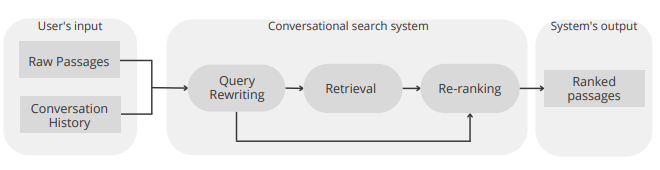
\includegraphics[width=7cm]{pipeline.png}
    \caption{Global Pipeline architecture of the system}
    \label{figure:1}
\end{figure}\\
  This will be similar to the architecture in Figure 1, which serves as the basis for the implementation of our baseline. The starting point of our project is therefore the list of input requests that will be submitted to the system. The main problem is to design a system which, according to a query, will perform a series of actions which will lead to the processing of this query, the evaluation of the most relevant documents and the display of the first 1000 documents. So we need to establish the different steps that will allow us to achieve this:\\
- Creation of the index from the collection of documents provided.\\
- A step of processing the query including a rewriting of it to be able to better process it.\\
- A step of searching for the most relevant documents through the document collection.\\
- One or more re-ranking steps in order to seek an optimal result.\\


\section{Baseline Method}

Explain what you are taking as your baseline method, as well as why this is a reasonable baseline, and why you are making specific implementation choices.

\section{Advanced Method}

Explain what you are taking as your advanced method(s), as well as why this is a promising attempt to outperform the baseline method, and why you are making specific implementation choices.

\section{Results}

With tables and graphs, make a clear, concise, and digestible presentation of the data produced by your experiments. This includes describing the key facts and trend from your results.


\begin{figure}[h]
    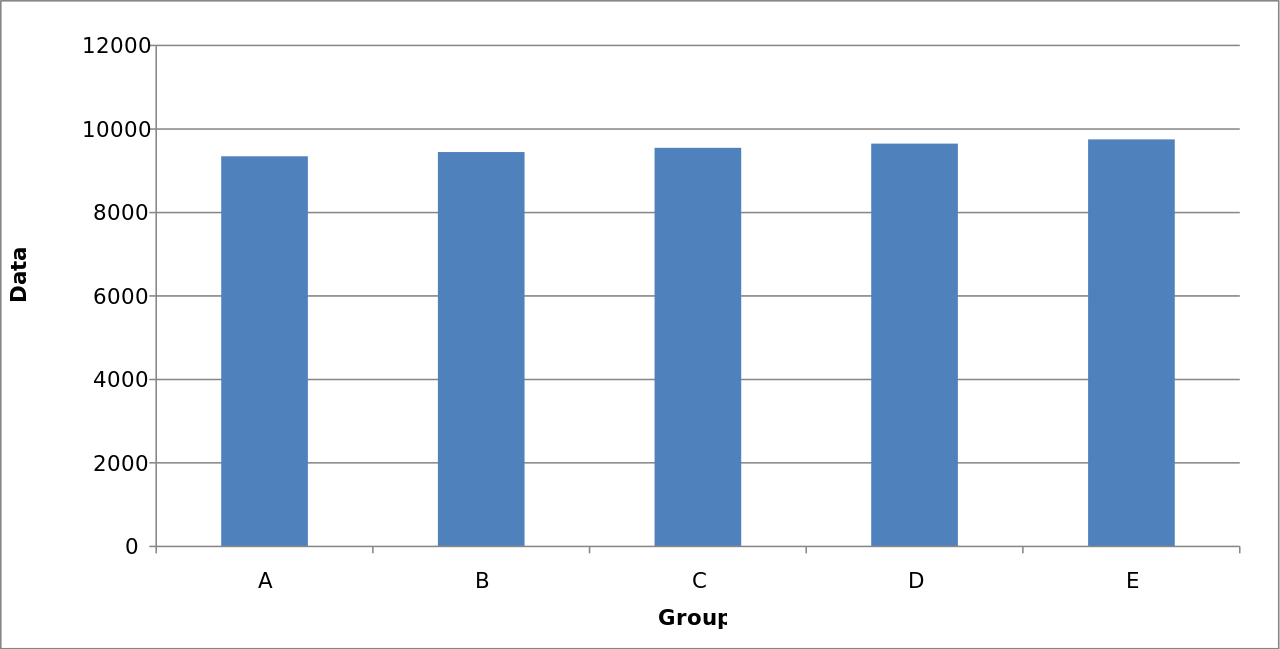
\includegraphics[width=6cm]{bar_graph.png}
    \caption{Figure caption}
    \label{figure:1}
\end{figure}


\begin{table}[h]
\begin{center}
\caption{Example table}
\begin{tabular}{l|rr}
     & Metric 1 & Metric 2 \\
    \hline
    Baseline 1 &  3 & 4 \\
    Baseline 2 &  3 & 3   \\
    Advanced Method 1 & 4 & 5 \\
    Advanced Method 1 & \textbf{5} & \textbf{6} 
\end{tabular}
\label{table:1}
\end{center}
\end{table}

\section{Discussion and Conclusions}

Summarize and discuss different challenges you faced and how you solved those. Include interpretations of the key facts and trends you observed and pointed out in the Results section. Which method performed best, and why? Speculate: What could you have done differently, and what consequences would that have had?

%%
%% If your work has an appendix, this is the place to put it.
%\appendix

%\section{Appendix}


%%
%% The next two lines define the bibliography style to be used, and
%% the bibliography file.
\bibliographystyle{ACM-Reference-Format}
\bibliography{base}

\newpage
\appendix
\section{Division of Work During the Project}

\end{document}
\endinput
